\chapter{Brief Introduction to Cosmology}

By the late part of the 20th century, the standard model of Cosmology
seemed to rest on firm foundations.  The model, known as the Cold Dark Matter
(CDM) model, consisted of a uniformly
expanding universe, comprised of baryonic matter, cold
non-baryonic (dark) matter, and radiation, with space-time evolving
according to the dynamics of Einstein's Theory of General Relativity.
This dynamical description, as was realized by Alexander Friedmann,
George Lemaitre, Howard Robertson, and Arthur Walker during the
1920s and 1930s,
predicts a dynamic universe, where space itself must expand or contract
under the influence of the energy within it.  The expansion of the universe,
first observed via the characteristic redshifts of distant galaxies
\citep{hubble1929}, was thought to be slowing under the
gravitational effect of the the matter within it.

This uniform expansion of space-time indicated that the early universe
was filled with a hot, dense plasma from which the constituents of
chemical elements
formed.  This theory of {\it Big Bang Nucleosynthesis} \citep[BBN:][]{Alpher48}
was and remains extremely successful in explaining the relative
abundance of chemical elements in the universe.  Another important prediction
within the BBN model is that a Cosmic Background Radiation should be present,
due to the photons which free-streamed once the universe cooled enough for
the gas within it to no longer be ionized \citep{Alpher48b}.
The CBR signal had been observed in detail \citep{Smoot92},
resulting in a confirmation of the inflationalry
hypothesis and the standard model of cosmology.

Nonetheless, the standard model had some cracks in its foundation:
cosmological probes and
studies of collapsed structures yielded widely discrepant estimates of the
matter content in the universe.  The implied age of the universe in the CDM
model was younger than the age inferred for the oldest observed globular
clusters and white dwarfs.  Something needed to change.

Observations of type Ia supernovae by \citet{Riess98}, and confirmed by
\citet{Perlmutter99} offered a solution: these showed that distant supernovae
were fainter than expected in a standard CDM model.  This implied that the
expansion of the universe was accelerating, due to a cosmological component
dubbed {\it dark energy}.  This dark energy has an effective negative pressure,
which overcomes the gravitational attraction of matter and causes the
expansion of space to accelerate.  This additional energy component in the
universe solved many of the problems posed by CDM, and is now part of the
standard $\Lambda$-CDM cosmological model ($\Lambda$ refers to the cosmological
constant first proposed by Einstein).

Led by these supernova results, as well as new observations of the cosmic
microwave background \citep[CMB;][]{WMAP1}, the baryon acoustic oscillations
\citep[BAO;][]{Eisenstein05}, and other observational
campaigns, the last 15 years has seen a surge in precision cosmologial
measurements.
The dark energy postulated to explain supernova distances is now known
to make up over 70\% of the energy density of the universe, and have
an equation of state consistent with it being due to
vacuum energy or a cosmological constant \citep{Kessler2009, WMAP7}.
Future surveys in many diverse areas of astronomy are seeking to place even
tighter constraints, allowing greater insight into the nature and evolution
of dark energy.

With such a wide and diverse field as Cosmology, we can't hope to offer
a complete introduction of the relevant theory in this work.
For a more complete discussion, there
are several very well-written books available; much of the material
discussed below is taken from formalism developed more fully in these works
\citep[see, e.g.][]{peebles1993principles, peacock1999cosmological,
  ryden2003cosmology, longair2008galaxy}.
This chapter will cover the basic physical and mathematical background of
the physical study of cosmology.  We will begin with a discussion of the
FLRW metric (named for Friedmann, Lemaitre,
Robertson, and Walker) which describes the geometry of space-time.
Next we'll move on to define the Friedmann Equations, which condense
the field equations of Einstein's General Relativity to the basic pieces
needed to describe the dynamics of a globally homogeneous and isotropic
universe.  We will then briefly discuss the relevant theory behind
gravitational structure formation within this model.
This paves the way to relate theory to data, using observations
including cluster counts, correlation functions, and Fourier power spectra.
Finally, we will develop the equations describing gravitational lensing
in the weak limit, and show how weak lensing observations can be used
to gain insight into the parameters of our cosmological model.
Throughout, we'll point out the relevant observational work which supports
and constrains these theories.

\section{FLRW Metric}
\label{sec:FLRW}
The physical study of cosmology in its classical form
is based on the fundamental assumption of symmetry:
that the universe on the largest scales is homogeneous and isotropic.
Homogeneity is an expression of translational symmetry: the appearance of
the universe does not depend on the location of the observer.  Isotropy
is an expression of rotational symmetry: the appearance of the universe
does not change with respect to the orientation of the observer.
These assumptions are clearly incorrect at small scales -- our galaxy
has a much higher density of stars in the central bulge than in the
outer halo, for example -- but they appear to hold at
the largest scales.
At distance scales larger than the size of typical superclusters
(about 50 Mpc or more), the distribution of
quasars and galaxies reflect the nearly homogeneous and isotropic
nature of large scale structure \citep{Yadav2005, Sarkar2009}.
More importantly, the Cosmic Microwave
Background appears homogeneous and isotropic to within one part in
$10^5$, giving evidence that our assumptions of homogeneity and isotropy
are well-founded for the universe as a whole \citep[For an interesting
discussion of the limits of this approach, however, see][]{Maartens2011}.

The most general metric for a homogeneous and isotropic space-time is due
to Howard Robertson and Arthur Walker, who showed that the space-time
distance $ds$ in spherical coordinates is given by
\begin{equation}
  \label{eq:FLRW_metric}
  ds^2 = -c^2 dt^2 + a(t)^2\left[dr^2 + S_\kappa^2(r)d\Phi^2\right]
\end{equation}
where $t$ is the time coordinate, $r$ and $\Phi$ are comoving spherical
coordinates,
$a(t)$ describes the distance scale (which may be an arbitrary function
of $t$), and $S_\kappa^2(r)$ is the curvature term.  The curvature term
depends on the curvature, $\kappa$, which may be either $+1$, $-1$, or $0$:
\begin{equation}
  \label{eq:FLRW_curvature}
  S_\kappa(r) = \left\{
  \begin{array}{ll}
    R\,\sin(r/R) & \kappa = +1\\
    r & \kappa = 0\\
    R\,\sinh(r/R) & \kappa = -1
  \end{array}
  \right.
\end{equation}
where $R$ is the radius of curvature today.  Often, the curvature
sign $\kappa$ and radius $R$ are compactly expressed in a single curvature
parameter $k$, such that $\kappa = k/|k|$ and $R = |k|^{-1/2}$.

The Robertson and Walker derived the above metric
from purely geometric arguments.
An interesting aspect of this metric is the scale factor $a(t)$.  A general
homogeneous and isotropic universe is not necessarily static: it can be
expanding or contracting with time.  The detailed nature of this expansion
cannot be derived from purely geometric means: the description of the dynamics
of cosmic expansion comes from the field equations of Einstein's theory
of General Relativity.

\section{The Friedmann Equations}
\label{sec:friedmann}
The Robertson-Walker metric (eq.~\ref{eq:FLRW_metric})
is a purely geometric result,
where the scale factor $a(t)$ is arbitrary and unspecified.
Friedmann and Lemaitre had earlier independently derived this expression
from Einstein's field equations, with the addition of certain dynamical
constraints on the scale factor.  For this reason, the Robertson-Walker
metric is often referred to as the Friedmann-Robertson-Walker metric
or the Friedmann-Lemaitre-Robertson-Walker (FLRW) metric.
The general relativistic constraints on the scale factor $a(t)$
are compactly expressed by the Friedmann
equations\footnote{For a  derivation of the Friedmann
  equations from the field equations of general relativity,
  refer to \citet{peebles1993principles}}:
\begin{equation}
  \label{eq:friedmann_1}
  \left(\frac{\dot{a}}{a}\right)^2
  = \frac{8\pi G}{3c^2}\varepsilon
  + \frac{\Lambda}{3} - \frac{\kappa c^2}{a^2 R^2}
\end{equation}
\begin{equation}
  \label{eq:friedmann_2}
  \frac{\ddot{a}}{a}
  = -\,\frac{4\pi G}{3c^2}(\varepsilon + 3P) + \frac{\Lambda}{3}.
\end{equation}
Here the scale factor $a$ is understood to be a function of time, and the
dots represent derivatives with respect to time.
By convention, the scale factor at the present day is
chosen to be $a(t_0) = 1$.  $\varepsilon$ and $P$ are
the energy density and pressure of the mass-energy in the universe, and
$\Lambda$ represents the cosmological constant.
Equations~\ref{eq:friedmann_1} and \ref{eq:friedmann_2} are the first and
second Friedmann equations, respectively.  The third Friedmann equation
can be easily derived from the first two:
\begin{equation}
  \label{eq:friedmann_3}
  \dot{\varepsilon} = -3\,\frac{\dot{a}}{a}\,(\varepsilon + P).
\end{equation}
This expression is equivalent to the first law of thermodynamics
expressed for the universe as a whole.

\subsection{Time Dialation and Redshift}
General Relativity tells us
that light always travels along null geodesics, that is, the space time
interval in eqn.~\ref{eq:FLRW_metric} satisfies $ds = 0$.  For a light
beam with no angular deflection $d\Omega$, this gives
\begin{equation}
  dr = \frac{c}{a(t)} dt.
\end{equation}
If a beam of light is emitted at time $t_e$ and travels
a comoving distance $r$, the
time $t_o$ that the light is observed can be found by solving
\begin{equation}
  r = \int_{t_e}^{t_o} \frac{c}{a(t)} dt
\end{equation}
If a second photon is emitted a short time later at time $t_e + \Delta t_e$,
and arrives at time $t_o + \Delta t_o$, this gives
\begin{eqnarray}
  r &=& 
  \int_{t_e + \Delta t_e}^{t_o + \Delta t_o} \frac{c}{a(t)} dt \nonumber\\
  &\approx& \int_{t_e}^{t_o} \frac{c}{a(t)} dt + \frac{c\Delta t_o}{a(t_o)}
  - \frac{c\Delta t_e}{a(t_e)},
\end{eqnarray}
where we have used a first-order approximation.  Equating these
two expressions gives for small $\Delta t$:
\begin{equation}
  \label{eq:time_dialation}
  \Delta t_o = \Delta t_e \frac{a(t_o)}{a(t_e)}.
\end{equation}
In an expanding universe, the observed time interval is longer than
the time interval in the emitted frame.  This {\it time dialation} is
a general feature of space-time governed by Einstein's field equations.

The time dialation has an observable effect on emitted light:
if an atom emits light with a period 
$P_e = \Delta t_e = \lambda_e / c$, then the observed wavelength $\lambda_o$
and the emitted wavelength $\lambda_e$ are related by
\begin{equation}
  \lambda_o = \lambda_e \frac{a(t_o)}{a(t_e)}.
\end{equation}
The wavelength of light is lengthened due to the expansion of space.  For
historical reasons, this expansion is generally parametrized using the
redshift:
\begin{equation}
  1 + z \equiv \frac{a(t_o)}{a(t_e)}.
\end{equation}
Because we define $a(t_o) = 1$, we have
\begin{equation}
  a(t_e) = \frac{1}{1 + z}.
\end{equation}
Thus the redshift of a light source gives us a direct measurement of the
scale factor at the time that photon was emitted.  As such, it can be
substituted for $a$ as the dependent variable in the above equations
with a suitable change-of-variables; we will switch between these two
conventions depending on which is convenient.

\subsection{Equation of State}
The Friedmann equations can be further simplified
by relating the pressure $P$ and energy
density $\varepsilon$ in terms of a linear equation of state parameter
\begin{equation}
  \label{eq:w_EOS}
  w \equiv P / \varepsilon.
\end{equation}
Using this, the solution of eqn.~\ref{eq:friedmann_3} gives
\begin{equation}
  \label{eq:w_constant}
  \varepsilon = \varepsilon_0\, a^{-3(1 + w)}
\end{equation}
for $w$ constant in time.
Here $\varepsilon_0 = \varepsilon(t_0)$ is the energy density today,
and we have used the standard convention $a(t_0) = 1$.
Given this parametrization, we can now
separate the various contributions to the mass-energy of the universe
and re-write eqn.~\ref{eq:friedmann_1} in terms of the equation of
state for each:
\begin{equation}
  \label{eq:friedmann_1_split}
  \left(\frac{\dot{a}}{a}\right)^2 = \frac{8\pi G}{3c^2}
  \sum_w \varepsilon_{w, 0} \,\, a^{-3(1 + w)}
\end{equation}
where $\varepsilon_{w,0}$ is the energy density of each species at present.
The various possible contributions are:
\begin{description}
  \item[Vacuum energy/Cosmological Constant:]
    The vacuum energy or cosmological constant $\Lambda$ has
    energy density which does not change with time.
    So by Equation~\ref{eq:friedmann_3}, $P = -\varepsilon$ and $w = -1$.
  \item[General Quintessence:] Quintessence is defined as any sort of matter
    or energy field
    which can balance the gravitational attraction, leading to accelerated
    expansion.  By Equation~\ref{eq:friedmann_2}, $\ddot{a}/a > 0$ only
    if $w < - 1/3$.  We see that the cosmological constant is a form of
    quintessence.
  \item[Curvature:] Though it may seem strange to think about the curvature
    of space as having an energy density, in General Relativity the curvature
    is in some sense a stand-in for gravitational potential energy.  Comparing
    eqns.~\ref{eq:friedmann_1} and \ref{eq:friedmann_1_split}, the dependence
    of the curvature term on scale factor $k \propto a^{-2}$
    means it has an effective equation
    of state parameter $w = -1/3$.  This makes it clear why curvature does
    not appear in the second Friedmann equation (eqn.~\ref{eq:friedmann_2}):
    for $w=-1/3$, $\varepsilon + 3P = 0$, and the presence of curvature
    cannot lead to a change in the expansion rate.
  \item[Non-relativistic matter:] Non-relativistic matter (often known
    as {\it cold matter}) has kinetic energy much less than its rest mass;
    in other words $P \sim kT \ll \varepsilon$.  This corresponds to
    $w \ll 1$, and we will often approximate this as simply $w=0$.
  \item[Relativistic Matter:] Relativistic matter 
    (known as {\it warm matter} or {\it hot matter}) has energy given by
    $E^2 = p^2c^2 + m^2 c^4$, where $p$ is the total momentum and $m$ is
    the rest-mass.  If $pc \ll mc^2$, we have the non-relativistic
    case above, and find $w \to 0$.  If $pc \gg mc^2$, then in analogy to
    the radiation case discussed below, we find $w \to 1/3$.
    For general relativistic matter, this leads to
    $0 \le w \le 1/3$, with the exact value dependent on the energy density.
  \item[Radiation:] Radiation has energy per particle
    proportional to the momentum times the speed of light.  From basic
    electrodynamics, one can show that for an ideal photon gas, each spatial
    degree of freedom contributes equally to the energy, so that the pressure
    is $P = dp/dt = \varepsilon / 3$.  So relativistic mass-energy has
    $w = 1/3$.
\end{description}

\subsection{Evolving Equation of State}
In Equation~\ref{eq:w_constant} we show the solution of
eqn.~\ref{eq:friedmann_3} for constant $w$.  Another possibility
(especially applicable for general quintessence models) is that
the equation of state parameter $w$ evolves with time.
\begin{equation}
  \label{eq:w_general}
  \varepsilon(a) = \varepsilon_0\, \exp\left[-3\int_1^a
    \frac{1 + w(a^\prime)}{a^\prime}\dd a^\prime\right].
\end{equation}
Many parametrizations of the form of $w(a)$ have been proposed.  Perhaps
the simplest is a model which is simply linear in the redshift $z$, i.e.
\begin{equation}
  w(z) \approx w_0 + w_1 z.
\end{equation}
Though simple, this parametrization is encumbered by the fact that $z$ changes
very quickly with time, especially in the early universe.  A better 
choice is the CPL parametrization \citep{Chevallier01, Linder03a}, which is
of the form
\begin{equation}
  w(z) \approx w_0 + w_a\frac{z}{1 + z},
\end{equation}
or equivalently
\begin{equation}
  w(a) \approx w_0 + w_a(1 - a)
\end{equation}
which is linear in the scale factor rather than the redshift.  Adopting this
parametrization gives
\begin{equation}
  \label{eq:w_first_order}
  \varepsilon(a) = \varepsilon_0\, a^{-3(1 + w_0 + w_a)}e^{-3w_a(1-a)}.
\end{equation}
One of the main goals of future cosmological surveys is to put meaningful
constraints on the time-evolution of dark energy, often by placing constraints
on $w_1$ or $w_a$.  This will be discussed further in later sections.

\subsection{Hubble Parameter}
\label{sec:hubble_parameter}
The first Friedmann equation (eqn.~\ref{eq:friedmann_1}) is commonly expressed
in terms of dimensionless parameters via the generalization in
eqn.~\ref{eq:friedmann_1_split}.  If we define the Hubble parameter
\begin{equation}
  \label{eq:hubble_parameter}
  H \equiv \frac{\dot{a}}{a},
\end{equation}
and let $H_0$ be the value of the Hubble parameter today, then
eqn.~\ref{eq:friedmann_1_split} becomes
\begin{equation}
  \left(\frac{H}{H_0}\right)^2 = \frac{8\pi G}{3H_0^2c^2}
  \sum_w \varepsilon_{w, 0} \,\, a^{-3(1 + w)}.
\end{equation}
The constant in front of the sum has dimensions of inverse energy density:
this motivates the definition of the critical density
\begin{equation}
  \label{eq:critical_density}
  \varepsilon_c \equiv \frac{\rho_c}{c^2} \equiv \frac{3 H^2 c^2}{8\pi G},
\end{equation}
where, to be explicit, both the critical densities $\varepsilon_c$,
$\rho_c$,
and Hubble parameter $H$ are functions of time.
With this definition, and defining the dimensionless density parameter
\begin{equation}
  \label{eq:density_parameter}
  \Omega_w(t) \equiv \varepsilon_w(t) / \varepsilon_c(t)
\end{equation}
the Friedmann equation can be compactly expressed
\begin{equation}
  \left(\frac{H}{H_0}\right)^2
  = \sum_w \Omega_{w, 0}\,\, a^{-3(1 + w)},
\end{equation}
where the subscript $0$ indicates the value at present.
Alternatively, we can express the Friedmann equation as simply
\begin{equation}
  \sum_w \Omega_w(t) = 1.
\end{equation}
Neglecting curvature, if the sum of components $\Omega_w$ is unity, then
we must have curvature $\Omega_\kappa = 0$.  This shows the meaning of
the critical density (eqn.~\ref{eq:critical_density}): if the energy density
in the universe satisfies $\epsilon > \epsilon_c$ (i.e. $\Omega > 1$), then
$\kappa = +1$ and the universe is {\it spatially closed}.
If $\epsilon < \epsilon_c$ (i.e. $\Omega < 1$), then $\kappa = -1$ and
the universe is {\it spatially open}. If the energy density is
exactly equal to the critical density, then the curvature $\kappa = 0$
and the universe is {\it flat}.  Constraints from the Cosmic Microwave
Background show that our universe is flat to a very high precision
\citep{WMAP7}.  For this reason, in many of the below derivations we will
assume for simplicity that $\Omega_\kappa = 0$ and $S_\kappa(r) = r$.

For simplicity, we can limit our consideration to the principal contributors
to the density of the universe:
dark energy $(\Omega_\Lambda)$, matter $(\Omega_M)$, radiation $(\Omega_R)$,
and curvature $(\Omega_\kappa)$.  Neglecting other components gives the
familiar dimensionless form of the Friedmann Equation:
\begin{equation}
  \label{eq:friedmann_dimensionless}
  \left(\frac{H}{H_0}\right)^2
  = \Omega_{M,0}\,\,a^{-3} + \Omega_{R,0}\,\,a^{-4}
  + \Omega_{\kappa,0}\,\,a^{-2} + \Omega_\Lambda
\end{equation}

\section{Cosmological Distance Measures}
\label{sec:distances}
The FLRW metric of \S\ref{sec:FLRW} and the Friedmann equations of
\S\ref{sec:friedmann} lay the basic framework for the study of cosmology.
A large portion of
the history of $20^{\rm th}$ century cosmology surrounds various
attempts to understand the relative contributions of matter, radiation,
curvature, and dark energy to the Hubble parameter, which measures
the expansion rate of the universe.  The exact nature of these various
contributions has far-reaching consequences,
determining how, when, and where galaxies, clusters and other structure
form and evolve; determining the age of the universe and the character of
its evolution through time; determining cosmic abundances and 
the initial conditions of stellar evolution
and planet formation; and determining the nature of the universe's beginning,
and the possibility of its eventual end.
Observational measures of these consequences allow constraints of the
properties of the various $\Omega_w(z)$.

Eqn.~\ref{eq:friedmann_dimensionless} is simply a first-order differential
equation in $a$: For various choices of the density parameters $\Omega_w$, it
can be solved to yield a curve describing the scale factor $a$ as a function
of time $t$.  A straightforward route to placing
observational constraints on the densities of
various components, then, would require simply measuring the value of $a$ at
several times $t$ and performing a multidimensional fit to these observed
data points.

As discussed above in \S\ref{sec:redshift}, the redshift of
light offers a direct measurement of the scale factor at a given time.
In order to use eqn.~\ref{eq:friedmann_dimensionless} to gain information
about the cosmological densities $\Omega_w$, then, we must be able to
observe some property related to the time $t_e$ of emission of these photons.
To enable this, we'll introduce the concept of distances in Cosmology.

Distance measures in cosmology are a potentially confusing subject.  An
excellent resource describing these can be found in \citet{hogg1999distance}.
Here we'll briefly define four relevant distance measures: the comoving
distance, the proper distance, the angular diameter distance, and the
luminosity distance.

\begin{description}
  \item[Comoving Distance:] The comoving distance is the distance $r$ which
    enters into the FLRW metric, eqn.~\ref{eq:FLRW_metric}.  This distance is
    constant for an object moving with the expansion of space.  Using the
    FLRW metric and setting $ds=0$, one can shown that the comoving
    distance for an object with redshift $z$ is given by
    \begin{equation}
      \label{eq:comoving_distance}
      r(z) = c\,\int_0^z \frac{dz^\prime}{H(z^\prime)}.
    \end{equation}
  \item[Proper Distance:] The proper distance $d_p(z)$ is the simultaneous
    separation between two objects.  From the FLRW metric with time interval
    $dt=0$, one can show that the proper distance is given by
    \begin{equation}
      \label{eq:proper_distance}
      d_p(z) = \frac{r(z)}{1 + z}.
    \end{equation}
  \item[Angular Diameter Distance:] The angular diameter distance $d_A(z)$
    is the
    ratio of the proper size to the observed angular size (in radians) of
    an extended source.  From the FLRW metric with $dt = dr = 0$, one
    can show that the angular diameter distance is given by
    \begin{equation}
      \label{eq:angular_diameter_distance}
      d_A(z) = \frac{S_\kappa(r)}{1 + z}.
    \end{equation}
  \item[Luminosity Distance:] The luminosity distance $d_L(z)$ relates the
    emitted flux of a source to the observed flux.  Taking into account
    the angular dilution of the flux, as well as the redshifted energy of
    each photon and time-delay of photon arrival leads to
    \begin{eqnarray}
      \label{eq:luminosity_distance}
      d_L(z) &=& (1 + z)^2\,d_A(z) \nonumber\\
      &=& (1 + z)\,S_\kappa(r)
    \end{eqnarray}
\end{description}
By measuring one of these distances as a function of redshift, we are
effectively measuring both the dependent and independent variable
in the dimensionless Friedmann equation, eqn.~\ref{eq:friedmann_dimensionless}.
In this way, it is possible to constrain the combinations of cosmological
parameters $\Omega_w$ which fit the data.

\section{Standard Candles: Cosmology via Luminosity Distance}
\label{sec:std_candles}
{\it Standard candles} have been one of the primary methods for measuring
cosmological parameters.  The earliest measure, from Edwin Hubble,
used Cepheid-type variable stars which have an absolute magnitude correlated
with their pulsation period \citep{hubble1929}.
Through observations of Cepheids
in nearby galaxies, Hubble found a positive correlation between the
luminosity distance to each galaxy and its apparent recessional velocity,
indicating a positive value for $H_0$.\footnote{
Although Hubble does not frame this measurement in terms of the Friedmann
equations, he cautiously mentions the potential relationship of the
observations to the ``de Sitter effect'', a predicted redshift within
a particular solution of
Einstein's equations which is a special case of the FLRW metric and
Friedmann equations (i.e., that with $\Omega_M = 0$, $\Omega_\kappa = 0$,
and $\Omega_\Lambda = 1$).}
Using our formalism above, we can show that the rate of change of the
proper distance to any object is
\begin{eqnarray}
  \frac{d}{dt}d_p(t) &=& H(t)\,\, d_p(t) \nonumber\\
                     &\approx& H_0\,\, d_L(t) \left[1 + \mathcal{O}(z)\right],
\end{eqnarray}
where in the second line we have separated corrections of order $z$.  Because
Hubble used a sample with $z <\sim 0.005$, the zeroth-order
linear fit is well within observed errors.
Thus Hubble's observations can be seen as a first attempt at constraining
cosmological parameters in Equation~\ref{eq:friedmann_dimensionless} through
the simultaneous measurement of redshift and luminosity distance.

In the 70 years after Hubble's discovery, there were many attempts to
confirm and improve upon his discovery and use it to derive tighter
constraints on the slope $H_0$ of the Hubble relation.  A large majority
of these have
been based on standard or standardizable candles.  These standardizable
candles have been based on several empirical relations, including
the period-luminosity relationship of Cepheid
variables \citep{Leavitt1912}; on the Tully-Fisher relationship between
brightness and rotation speed of spiral galaxies \citep{Tully77}; on
the Faber-Jackson/Fundamental Plane relationship between brightness,
velocity, and surface brightness for elliptical galaxies
\citep{Faber76, Djorgovski87}; and on the relationship between luminosity
and decay timescale for type Ia supernovae \citep{Philips93}.  Due to
their extreme intrinsic brightness and minimal scatter in
calibrated luminosity, type Ia supernovae have become a very important
tool for determining cosmological parameters, but they cannot be used
alone: independent measures are required to calibrate the distance
scale of type-I supernovae, making all the above approaches important.
Perhaps the most comprehensive study to date of these various standard
candles is the HST Key project \citep{Freedman01}, which combined
the above measures and others to arrive
at a value of $H_0 = 72 \pm 8$ km/s/Mpc.  This is consistent with the
tighter constraint from the WMAP 7-year CMB analysis, which gave
$H_0 = 70.4 \pm 2.5$ km/s/Mpc.

The common theme in the above methods is that they are based on the idea
of a standard candle: if we can determine the intrinsic brightness
of an object as well as its redshift, then we can compare this to the
apparent brightness and constrain the Hubble parameter $H(t)$.
Another path to this sort of constraint comes from standard {\it rulers}
rather than standard candles.  If we know the redshift as well as the
intrinsic size of an object, then we can use its apparent size to
constrain cosmological parameters.  One such standard ruler is given by the
characteristic scales of structure in the universe.

\section{The Growth of Structure}
\label{sec:growth}
There are several methods of cosmological parameter estimation which rely
on the idea of standard rulers.  Some examples are the observation of the
anisotropy scale in the Cosmic Microwave Background, and the observation
of the Baryon Acoustic Oscillation scale.
Another powerful method relies on detailed modeling of the growth of structure.
As we will see, along with offering the possibility of a standard ruler,
consideration of structure growth can offer other cosmologically interesting
observables.

The distribution of density throughout the universe can be expressed
in terms of the density contrast
\begin{equation}
  \label{eq:overdensity}
  \delta(\myvec{x}, t) = \frac{\rho(\myvec{x}, t) - \rho_b(t)}{\rho_b(t)},
\end{equation}
where the background matter density is
\begin{equation}
  \rho_b(t) \propto \frac{1}{a(t)^3}
\end{equation}
(i.e.~we assume the background consists of cold matter with $w=0$).
Rearranging this definition results in expressing the density field of the
universe as
\begin{equation}
  \rho(\myvec{x}, t) = \rho_b(t)[1 + \delta(\myvec{x}, t)].
\end{equation}

\subsection{Gravitational Instability}
We can proceed by treating matter as an ideal fluid with a
velocity field $\myvec{u}(\myvec{x}, t)$ and pressure $P(\myvec{x}, t)$
\citep{longair2008galaxy}.
In this case, it is governed by three equations: the
continuity equation, which describes conservation of mass,
\begin{equation}
  \label{eq:continuity}
  \left(\frac{\partial\rho}{\partial t}\right)_{\myvec{x}}
  + \rho\myvec{\nabla}_{\myvec{x}}\cdot\myvec{u} = 0,
\end{equation}
the Euler equation, which specifies conservation of momentum,
\begin{equation}
  \label{eq:euler}
  \left(\frac{\partial\myvec{u}}{\partial t}\right)_{\myvec{x}}
  + (\myvec{u}\cdot\myvec{\nabla}_{\myvec{x}})\myvec{u}
  + \frac{\myvec{\nabla}_{\myvec{x}}P}{\rho}
  = -\myvec{\nabla}_{\myvec{x}}\Phi,
\end{equation}
and the Poisson equation, which describes gravity in the Newtonian limit
\begin{equation}
  \label{eq:poisson}
  \nabla_{\myvec{x}}^2\Phi = 4\pi G\rho.
\end{equation}
Transforming to comoving coordinates $\myvec{r} = \myvec{x}/a(t)$,
defining comoving time derivatives
$d/dt \equiv \partial/\partial t + \myvec{u}\cdot\myvec{\nabla}$,
and expressing in terms of the dimensionless density contrast
$\delta(\myvec{r}, t)$ (eq.~\ref{eq:overdensity}) gives
\begin{equation}
  \label{eq:delta_evolution}
  \frac{d^2\delta}{d t^2} + 2 H \frac{d\delta}{d t}
  = \frac{c_s^2}{a^2}\nabla_{\myvec{r}}^2\delta + 4\pi G \rho_b\,\delta
\end{equation}
where $\nabla^2_{\myvec{r}}$ indicates the Laplacian with respect to comoving
coordinates \citep[for derivation see section 11.2 of][]{longair2008galaxy}.

We can gain insight by expressing this in terms of
wave-like solutions of the denstity contrast
$\delta_k(\myvec{r}, t) \propto \exp[i(\myvec{k}\cdot\myvec{r} - \omega t)]$,
where $\myvec{k}$ is the vector of spatial wave-numbers, and $\omega$
is the oscillation frequency.  In terms of these Fourier modes,
eqn.~\ref{eq:delta_evolution} becomes
\begin{equation}
  \label{eq:delta_evolution_k}
  \ddot{\delta}_k + 2 H \dot{\delta}_k - \delta_k(4\pi G\rho_b - k^2c_s^2) = 0.
\end{equation}
This differential equation describes an exponentially growing (or decaying)
density fluctuation, with a ``drag'' term governed by the Hubble parameter
$H(z)$.  The rate of growth of perturbations $\delta_k$ depends
on the balance between the gravitational force through $4\pi G\rho_b$ and the
pressure through $k^2c_s^2$.  The scale $\lambda_J = 2\pi/k_J$
where these forces balance is called the Jeans length:
\begin{equation}
  \label{eq:jeans_length}
  \lambda_J \equiv c_s \sqrt{\frac{\pi}{G\rho_b}}.
\end{equation}
This is the scale above which pressure cannot halt gravitational
collapse.  The length is directly proportional to the sound speed
$c_s = \sqrt{\partial P/\partial \rho}$ and so depends on the equation of
state of the total energy in the universe,
as well as the average density $\rho_b$.
The different components (radiation, matter, etc.) have different
equations of state (\S\ref{sec:friedmann}) and evolve
with different dependencies on the scale factor
$a$, and so the Jeans length also evolves through the course of cosmic
history.  Thus the scale of nonlinear
collapsed structure as a function of $z$ contains information which can
be used to place constraints on the components which make up the Universe.

In particular, we can consider two relevant regimes: radiation dominance
and matter dominance.  In the regime where radiation dominates the energy
density, the equation of state $w=1/3$ leads to $c_s^2 = c^2/3$.  In a flat
universe $\rho_b$ is the critical density (eqn.~\ref{eq:critical_density})
and the Jeans length for a radiation dominated universe can be expressed
\begin{equation}
  \label{eq:jeans_radiation}
  \lambda_J^{(R)} = \frac{\pi c \sqrt{8}}{3 H}.
\end{equation}
This scale is on the same order as that of the horizon scale,
$\lambda_s \approx 2c / (H\sqrt{3})$.  This means that sub-horizon modes
cannot collapse during the epoch when radiation dominates the energy
of the universe.

In the matter-dominated regime, there are two possibilities: if radiation and
matter are coupled, the pressure comes from the radiation
while the density is dominated by matter.  This gives
$c_s^2 \sim c^2 \Omega_r / \Omega_M \sim c^2 (1 + z)
\Omega_{r,0}/\Omega_{m, 0}$.
Putting in numbers from WMAP \citep{WMAP7}, we find approximately
$c_s \approx 10^{-2} c \sqrt{1 + z}$.
If radiation and matter are decoupled, the pressure comes from the nonzero
temperature of matter itself:
$c_s^2 \sim kT/m_p$ where $m_p$ is the proton mass.  Assuming the matter
is in thermal equilibrium with the CMB, then temperature goes as
$T \propto (1 + z)$.  Again using observational constraints from WMAP, we find
$c_s \approx 10^{-7} c \sqrt{1 + z}$.  Thus the Jeans length during the
matter-dominated epoch is given by
\begin{equation}
  \label{eq:jeans_matter}
  \lambda_J^{(M)} \approx \lambda_J^{(R)}\sqrt{1 + z}\,\, \times \left\{
  \begin{array}{ll}
    10^{-2} & \mathrm{before\ decoupling}\\
    10^{-7} & \mathrm{after\ decoupling}
  \end{array}
  \right.
\end{equation}
The redshift of decoupling is approximately $z \sim 1100$ \citep[for a physical
argument for this, see][]{ryden2003cosmology}.  This means that prior to
decoupling, growth below approximately sub-horizon scales is suppressed by
pressure.  After decoupling, the Jeans length shrinks by five orders of
magnitude, allowing linear structure on this scale to form.  The observable
effect of this sharp transition in the growth of structure will be discussed
further below.

A related question is that of the rate of structure growth
on scales larger than the Jeans length. 
This can be addressed by defining the linear growth
factor $D(t)$ such that
\begin{equation}
  \label{eq:linear_growth_def}
  \delta(\myvec{r}, t) = \delta_0(\myvec{r})D(t).
\end{equation}
Using $\rho_b = \Omega_M\rho_c$ and assuming negligible pressure (i.e. scales
above the Jeans length), we can rewrite
eqn.~\ref{eq:delta_evolution} as
\begin{equation}
  \label{eq:linear_growth_eqn}
  \ddot{D} + 2H\dot{D} - \frac{3}{2}\Omega_M H^2D = 0.
\end{equation}
This is a second-order differential equation, which will, in general,
admit a solution with a growing mode and a decaying mode:
\begin{equation}
  D(t) = A_1 D_1(t) + A_2 D_2(t).
\end{equation}
In a flat universe dominated by matter, the
Friedmann equation gives $H(t) = 2 / (3t)$, leading to solutions
\begin{equation}
  D(t) = A_1 t^{2/3} + A_2 t^{-1}.
\end{equation}
The first term quickly dominates the second, and structure grows as
$\delta \propto t^{2/3} \propto a$, where the last proportionality comes
from solving eqn.~\ref{eq:friedmann_dimensionless} for a matter dominated
universe.

In general, the growth factor for a flat universe is
\begin{equation}
  \label{eq:linear_growth}
  D(a) \propto \int_0^a \frac{da^\prime}{[a^\prime H(a^\prime)]^3},
\end{equation}
where the normalization is usually chosen such that $D(a) = 1$ at the
present day.

A radiation-dominated universe presents a more complicated case:
eqn.~\ref{eq:linear_growth_eqn} assumes the pressure is negligible compared
to the gravitational force.  This approximation breaks down in
cases when $\Omega_M \to 0$.  For these cases, we need a more involved
perturbative treatment.

\subsection{Perturbation Treatment}
To explore the growth rate in a universe where $\Omega_M$ is small, we
will perform a perturbation analysis of Friedmann's equations.
A full discussion of this treatment can be found in
\citet{peebles1993principles}.
Here we will briefly outline a schematic approach from \citet{kolb_turner}
which leads to the same results.

By Birkhoff's theorem, a small spherical over-density can be treated as if
it were an independent homogeneous universe embedded within the background.
We'll assume the background is represented by a flat universe with
\begin{equation}
  H^2 = \frac{8\pi G}{3c^2}\varepsilon_0,
\end{equation}
and that a spherical perturbation has a small positive curvature
\begin{equation}
  H^2 = \frac{8\pi G}{3c^2}\varepsilon_1 - \frac{\kappa c^2}{a^2R_0^2}.
\end{equation}
The boundary requires that the expansion rate $H$ be equal between the
two; combining these we find
\begin{equation}
  \delta \equiv \frac{\varepsilon_1 - \varepsilon_0}{\varepsilon_0}
  = \frac{3\kappa c^4}{8\pi G R_0^2}\,\frac{1}{a^2 \varepsilon_0}.
\end{equation}
For a matter-dominated universe, $\varepsilon_0 \propto a^{-3}$
which gives $\delta \propto a$ as above.
For a radiation-dominated universe, $\varepsilon_0 \propto a^{-4}$
which gives $\delta \propto a^2$.

\subsection{Matter Power Spectrum}
In summary, the above results show that
\begin{itemize}
  \item In the radiation-dominated regime, fluctuations on scales above
    $\lambda_J^{(R)} = (\pi c \sqrt{8})/(3 H)$ grow as
    $\delta(a) \propto a^2$.
  \item In the matter-dominated regime, after decoupling, scales above
    $\lambda_J^{(M)}\approx 10^{-7} \lambda_J^{(R)} \sqrt{1 + z}$
    grow as $\delta(a) \propto a$.
\end{itemize}
The ratio of radiation density to matter density is
\begin{equation}
  \frac{\Omega_R(z)}{\Omega_M(z)} = (1 + z)\frac{\Omega_{R,0}}{\Omega_{M,0}}.
\end{equation}
So before the redshift of radiation-matter equality,
$z_{rm} \approx \Omega_{M,0}/\Omega_{R,0}$, radiation
dominates, while after this redshift matter dominates.
Thus the important scale is the horizon scale $\lambda_{rm}$ at
redshift $z=z_{rm}$.
Modes on length-scales $k > \lambda_{rm}$ will grow as $\delta \propto a^2$
for $a < a_{rm}$, and $\delta \propto a$ for $a > a_{rm}$.  Modes with
length-scales $k < \lambda_{rm}$ will grow as $\delta \propto a^2$ as long
as the horizon distance $d_{hor}(a) < k$, at which point the growth will
be suppressed by radiation pressure.  At $a > a_{rm}$, the Jeans length
shrinks by a factor of about $10^5$, and modes larger than $\lambda_J^{M}$
resume growth with $\delta \propto a$.

%\comment{add a picture of this here?}

Thus, density modes with $k < k_{rm}$ are suppressed by a factor of
$(a_k / a_{rm})^2 \propto k^{-2}$.  This motivates use of the power
spectrum of density fluctuations (for details see
Appendix~\ref{app:RandomFields}):
\begin{equation}
  \label{eq:power_spectrum}
  P_k \equiv \langle|\delta_k|^2\rangle,
\end{equation}
in theory a measurable quantity, which will have a distinct break at
$k = k_{rm}$ for the reasons discussed above.
In particular, if the power spectrum of primordial fluctuations
is a simple power law with $P_k \propto k^n$,
then after decoupling the power spectrum will be approximately
\begin{equation}
  P_k \propto \left\{
  \begin{array}{ll}
    k^{n-4}, & {\rm for\ } k < k_{rm} \\
    k^n, & {\rm for\ } k > k_{rm}.
  \end{array}
  \right.
\end{equation}
Under most inflationary scenarios, it is expected that the power spectral
index $n \approx 1$ \citep{peacock1999cosmological}.
The normalization of the power spectrum depends on the magnitude of the
primordial fluctuations, and is dependent on the cosmological model.
This normalization is typically expressed in terms of the parameter
$\sigma_8$, which measures the magnitude of average fluctuations within
a sphere of radius 8 Mpc.  For a more thorough discussion of power spectra
and the $\sigma_8$ normalization, see Appendix~\ref{app:RandomFields}.

\subsection{Putting it all together}
The sum of the above discussion paints a general picture of the growth of
structure within the universe presents several concepts with readily
observable consequences:

\begin{itemize}
  \item The size and mass/length scale of clusters as a function of redshift
    depends on the length-scale of gravitational instability $\lambda_J$
    (eqn.~\ref{eq:jeans_length}),
    which in turn depends on the densities of matter and radiation in the
    universe.  Clustering also depends on the linear growth rate
    $D(z)$ (eqn.~\ref{eq:linear_growth}) and its nonlinear extentions,
    which also depend on the relative cosmic densities as a function of $z$.
  \item The power spectrum of density fluctuations (eq.~\ref{eq:power_spectrum})
    has a turn-off at
    a length scale which is closely related to the horizon distance
    at the epoch of radiation-matter equality.  This scale acts as a standard
    ruler, such that the angular diameter distance can be estimated at a
    particular value of $z$, leading to cosmological constraints through the
    same means as the standard candle method discussed in
    \S\ref{sec:std_candles}.
  \item The linear growth factor (eqn.~\ref{eq:linear_growth}) affects the
    normalization of the power spectrum.  Therefore, measuring the power
    spectrum as a function of $z$ leads to cosmological constraints
    through the dependence of $D(z)$ on cosmological parameters.
\end{itemize}

So we see that there are powerful cosmological constraints which can be
obtained through the observation of the density fluctuations and clustering
of matter through the universe.  There are several caveats, however:
the above discussion focuses on the linear approximation (that is, we
discuss the behavior of perturbations of order $\delta$, while ignoring
$\delta^2$).  This is sufficient for small $\delta$, but not for when
$\delta$ is much larger than 1.  At small scales, structure is well beyond
the regime where this approximation holds: for example, $\delta$ for our
galaxy is approximately $10^5$!  Even moderate-sized galaxy clusters
(i.e. a hypothetical cluster 2Mpc across, containing 50 Milky-way
sized galaxies) has $\delta$ of order $10^2-10^3$.  Clearly, nonlinear
effects must be taken into account when measuring clustering.  These
effects can be estimated several ways; one of the more successful is the
halo model of \citet{Smith03}, which is calibrated using semi-analytic
results from N-body simulations.  Nonlinear effects lead to a significant
boosting of power on small scales.

A second caveat is that
the structure we are referring to here is that made up by the bulk
of the matter in the universe: collisionless dark matter.  Dark matter,
being non-luminous, cannot be obeserved directly through emitted light.
The power spectrum of luminous matter can be theoretically mapped to the
underlying mass power spectrum, but this mapping requires uncertain
corrections which introduces systematic errors which are difficult to
calibrate.

With careful accounting for the above two caveats, observations of the spatial
distribution of luminous matter has led to interesting cosmological results.
One of the most important surveys in this regard has been the Sloan Digital
Sky Survey (SDSS), which measured spectra of nearly a million sources across
over 8000 square degrees, leading to accurate photometric redshifts of
hundreds of thousands of galaxies across over a third of the sky.
Measurements of the angular power of these galaxies have been successfully
used to constrain cosmology both from the nonlinear power spectrum
\citep{Tegmark06} and the Baryon Acoustic Oscillation (BAO) signal
\citep{Eisenstein05}.

The BAO signal is another cosmological constraint based on the idea of a
standard ruler.  In the above discussion, we mention the role of pressure
in suppressing the growth of structure before radiation and matter are
decoupled.  This suppression by pressure leads to acoustic oscillations
in the plasma of the radiation and baryons.  When the radiation and matter
decouples, these oscillations freeze-out and form the seeds of baryonic
structure growth.  The remnants of this freeze-out can be observed in
baryonic structure today, and the characteristic length scale has been
used to place tight constraints on cosmological parameters
\citep{Eisenstein05}.

%\comment{ Should we also briefly mention WMAP anisotropies and the BAO signal?
%  They're essentially very accurate standard rulers at different epochs.
%  But I don't want to digress too much...}

\section{Gravitational Lensing}
\label{sec:gravitational_lensing}
In order to circumvent the astrophysical bias
involved with mapping luminous matter to
the underlying dark matter, it would be preferable to observe the dark
matter directly.  This is where gravitational lensing can be a
useful tool.
Einstein's theory of General Relativity predicts that photons will be deflected
in the presence of a gravitational field.  Under certain circumstances, this
deflection can be detected and used to learn about the nature of the
gravitating matter.

\subsection{Simplifying Assumptions}
\label{sec:lensing_simplification}
The propagation of light through a region of gravitational potential
$\Phi(\vec{r})$ is, in general, a very complicated\ problem, only analytically
solvable for potentials with various symmetries.  In cosmological contexts,
however, it is safe to assume that the universe is described by a
Robertson-Walker metric, with only small perturbations due to the density
fluctuations described by the potential $\Phi$.  In this case, the
gravitational deflection of a photon can be described by an effective
index of refraction given by
\begin{equation}
  n = 1-\frac{2}{c^2}\Phi 
\end{equation}
\citep[see][and references therein]{narayan1996lectures}.
As in conventional optics, light rays are deflected in proportion to the
perpendicular gradient of the refraction index, such that the deflection angle
$\hat{\alpha}$ is given by
\begin{equation}
  \label{eq:alpha-def}
  \hat{\alpha} = -\int_0^{D_S} \vec{\nabla}_\perp n \,\,\dd D
  = \frac{2}{c^2}\int_0^{D_S} \vec{\nabla}_\perp\Phi\,\,\dd D
\end{equation}
where $D_S$ is the distance from the observer to the photon source.  

For a point-mass located at a distance $D_L$ and an impact parameter $b$, with $D_L \gg b$ and $D_S \approx 2D_L$, equation \ref{eq:alpha-def} can be integrated to give
\begin{equation}
  \hat{\alpha} = \frac{4GM}{bc^2}\Bigg[1 - \frac{1}{2}\bigg(\frac{b}{D_L}\bigg)^2 + \mathcal{O}\bigg[\frac{b}{D_L}\bigg]^3 \Bigg]
\end{equation}
The first-order approximation is twice the deflection predicted by Newtonian gravity for a particle of arbitrary mass moving at a speed $c$.  It is important to note here that to first order, the deflection does not depend on the distance to the lens or source.  That is, for a mass distribution located at a distance $D_L \gg b$, equation \ref{eq:alpha-def} can be approximated
\begin{equation}
  \label{eq:alpha-def-approx}
  \hat{\alpha} \approx \frac{2}{c^2}\int_{D_L-\delta D}^{D_L+\delta D} \vec{\nabla}_\perp\Phi\,\dd D
\end{equation}
for $\delta D$ sufficiently greater than the size scale of the mass-distribution in question.
%Also note that for a large lens distance $D_L$, the contribution to $\hat{\alpha}$ becomes vanishingly small, and can be neglected.
So, to a very good approximation, the incremental deflection $\delta \hat{\alpha}$ of a photon at a given point along its trajectory is entirely due to a sheet of matter with a width $2\,\delta D$, oriented perpendicular to the unperturbed photon trajectory.  This is the {\it thin lens} approximation.

\subsection{Lensing Geometry}

\begin{figure}
  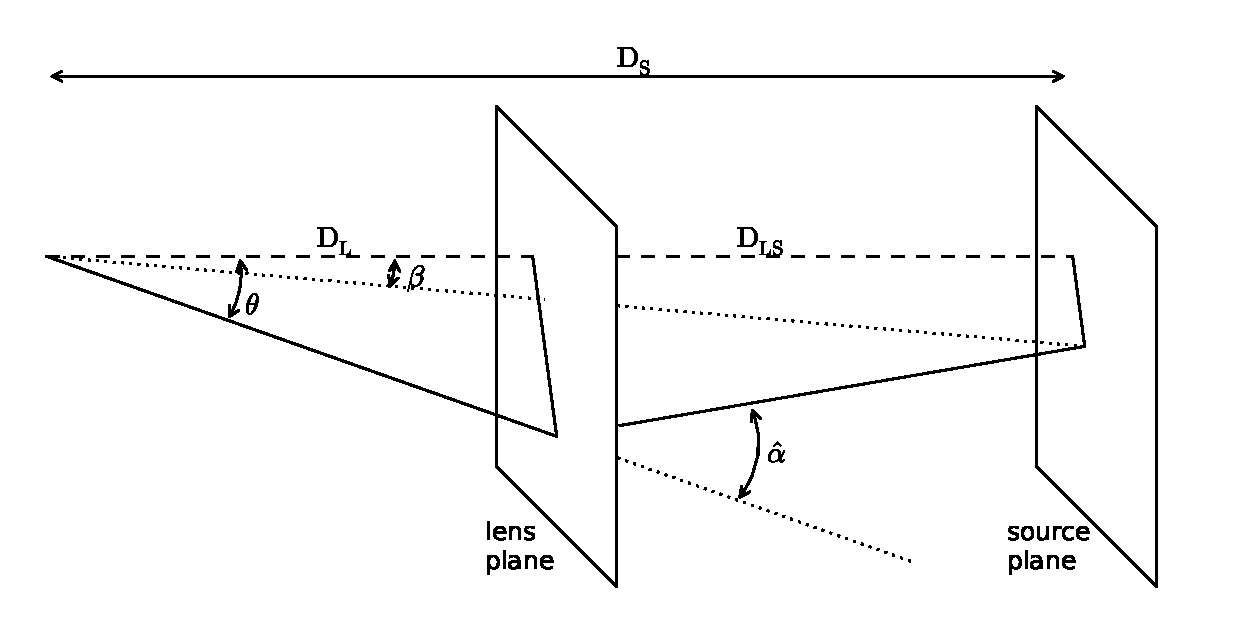
\includegraphics[width=\textwidth]{lensing_geometry.eps}
  \caption{The geometry of gravitational lensing}
  \label{fig:lensing_geometry}
\end{figure}

For a mass-sheet located at a distance $D_L$, and a photon source located at a distance $D_S$ (with $D_{LS} = D_S - D_L$) geometric considerations in the small-angle approximation (see Figure~\ref{fig:lensing_geometry}) yield the relation
\begin{equation}
  \vec{\theta} = \vec{\beta} + \frac{D_{LS}}{D_S}\hat{\vec{\alpha}}
\end{equation}
where $\vec{\theta}$ and $\vec{\beta}$ are the observed and true positions of the source, respectively.  Rescaling $\hat{\vec{\alpha}}$ in more convenient units gives
\begin{equation}
  \label{eq:mapping}
  \vec{\theta} = \vec{\beta} + \vec{\alpha}
\end{equation}
where we have defined
\begin{equation}
  \label{eq:alpha-def2}
  \vec{\alpha} \equiv \frac{D_{LS}}{D_S}\hat{\vec{\alpha}}
\end{equation}

\subsection{Continuous Mass Distribution}
In the case of a continuous mass distribution, we can recall the remarks of section \ref{sec:lensing_simplification}, and define a surface-mass density for a mass-sheet located at a redshift $z_L$:
\begin{equation}
  \label{eq:sigma-def}
  \Sigma(\vec{\theta},z_L) 
  = \int_{D_L-\delta D}^{D_L+\delta D}\rho_M(\vec{\theta},D)\dd D 
  = \frac{1}{c^2}\int_{z_L - \delta z}^{z_L + \delta z} 
  \varepsilon_M(\vec{\theta},z)\frac{dD}{dz}\dd z
\end{equation}
where $\varepsilon_M \equiv \rho_M c^2$ is the energy density of matter,
$\vec{\theta}$ is the apparent angular position, and $z$ and $D(z)$ are the 
redshift and line-of-sight distance, respectively, with $D_S = D(z_s)$.  

A matter distribution $\rho_M(\vec{\theta},z)$, and its Newtonian potential $\Phi(\vec{\theta},z)$ are related by Poisson's equation:
\begin{equation}
  \label{eq:poisson}
  \nabla^2 \Phi(\vec{\theta},z) = 4\pi G \rho_M(\vec{\theta},z)
\end{equation}

It is convenient to define the unscaled lensing potential $\hat{\psi}$, 
given by
\begin{equation}
  \hat{\psi}(\vec{\theta},z_s) 
  = \int_{0}^{D(z_s)} \Phi(\vec{\theta},z(D))\,\,\dd D 
  = \int_{0}^{z_s}\Phi(\vec{\theta},z)\frac{dD}{dz}\,\,\dd z
\end{equation}
Using the approximation in equation \ref{eq:alpha-def-approx}, we can write this in terms of multiple mass-sheets, such that
\begin{equation}
  \hat{\psi} = \sum_i \delta \hat{\psi}_i 
  = \sum_i \int_{D_i-\delta D}^{D_i+\delta D}\Phi \dd D
\end{equation}
with $D_{i+1} = D_i + 2\delta D$.

The gradient of $\hat{\psi}$ with respect to 
$\vec{\xi} \equiv D_L\vec{\theta}$ is
\begin{equation}
  \vec{\nabla}_\xi\hat{\psi} 
  = \sum_i \vec{\nabla}_\xi\big(\delta\hat{\psi}_i\big) 
  = \sum_i \int_{D_i - \delta D}^{D_i+\delta D}\vec{\nabla}_\xi \Phi \dd D
\end{equation}
Comparing this with (\ref{eq:alpha-def-approx}) and (\ref{eq:alpha-def2}) gives the incremental deflection angle in terms of the lensing potential of a mass-sheet:
\begin{equation}
  \delta\vec{\alpha}_i = \frac{2}{c^2}\frac{D_{LS}}{D_S}\vec{\nabla}_\xi (\delta\hat{\psi}_i)
\end{equation}
Further simplification can be made by rescaling the lensing potential,
defining
\begin{equation}
  \delta\psi_i = \frac{2}{c^2}\frac{D_{LS}}{D_L D_S} \delta\hat{\psi}_i
\end{equation}
so that we are left with
\begin{equation}
  \label{eq:alpha-psi}
  \delta\vec{\alpha}_i(\vec{\theta},z_L) = \vec{\nabla}_\theta \Big( \delta\psi_i(\vec{\theta},z_L)\Big)
\end{equation}
Defining the total scaled lensing potential $\psi = \sum_i \delta\psi_i$, and the total deflection $\vec{\alpha} = \sum_i\delta\vec{\alpha}_i$, we obtain
\begin{equation}
  \vec{\alpha}(\vec{\theta},z_s) = \vec{\nabla}_\theta \psi(\vec{\theta},z_s)
\end{equation}

The Laplacian of $\delta\psi_i$ with respect to theta is given by
\begin{equation}
  \nabla_\theta^2 (\delta\psi_i) 
  = \frac{2}{c^2}\frac{D_{LS}D_L}{D_S}\int_{D_L-\delta D}^{D_L+\delta D} 
  \nabla_\xi^2\Phi \dd D
\end{equation}
Using (\ref{eq:sigma-def}) and (\ref{eq:poisson}) this becomes
\begin{equation}
  \label{eq:psi-sigma_init}
  \nabla_\theta^2(\delta\psi_i) = \frac{8\pi G}{c^2}\frac{D_{LS}D_L}{D_S}\Sigma(\vec{\theta},z_i)
\end{equation}

We now define the critical surface density,
\begin{equation}
  \Sigma_{c}(z) \equiv\frac{c^2 D_S}{4\pi G D_L(z) D_{LS}(z)}
\end{equation}
and the convergence
\begin{equation}
  \label{eq:kappa-sigma}
  \kappa(\vec{\theta},z_s) \equiv \sum \frac{\Sigma(\vec{\theta},z_i)}{\Sigma_c(z_i)}\ \forall\ z_i < z_s
\end{equation}
Now summing all the mass-sheets in (\ref{eq:psi-sigma_init}) gives the relation between the scaled lensing potential and the convergence
\begin{equation}
  \label{eq:psi-kappa-1}
  \nabla_\theta^2\psi(\vec{\theta},z_s) = 2\kappa(\vec{\theta},z_s)
\end{equation}

Solving this two-dimensional differential equation gives the effective potential in terms of the convergence:
\begin{equation}
  \label{eq:psi-kappa}
  \psi(\vec{\theta},z) 
  = \frac{1}{\pi}\int_{\mathbb{R}^2} \kappa(\vec{\theta}^\prime,z) 
  \ln|\vec{\theta} - \vec{\theta}^\prime|\dd^2\theta^\prime
\end{equation}

\section{Weak Gravitational Lensing}

The local properties of the mapping in (\ref{eq:mapping}) are contained in its Jacobian matrix, given by
\begin{equation}
  \label{eq:Jacobian_def}
  \mathcal{A} \equiv \frac{\partial \vec{\beta}}{\partial \vec{\theta}} = \Big(\delta_{ij} - \frac{\partial \alpha_i}{\partial \theta_j} \Big) = \Big(\delta_{ij} - \frac{\partial^2 \psi}{\partial \theta_i \partial \theta_j} \Big),
\end{equation}
where $i,j$ index the two components of the angular position.

Introducing the abbreviation
\begin{equation}
  \label{eq:psi_ij}
  \psi_{ij} = \frac{\partial^2 \psi}{\partial \theta_i \partial \theta_j}
\end{equation}
We can then rewrite the convergence $\kappa$ (eqn \ref{eq:psi-kappa-1}) and define the complex shear $\gamma \equiv \gamma_1 + i\gamma_2$ of the mapping and write:
\begin{equation}
  \label{eq:gamma-def}
  \begin{array}{lcl}
    \kappa & = & (\psi_{11} + \psi_{22})/2\\
    \gamma_1 & = & (\psi_{11} - \psi_{22})/2\\
    \gamma_2 & = & \psi_{21} = \psi_{12}
  \end{array}
\end{equation}
The local Jacobian matrix (\ref{eq:Jacobian_def}) of the lens mapping can then be written
\begin{equation}
  \label{eq:jacobian_kappa_gamma}
  \mathcal{A} = \left(
  \begin{array}{cc}
    1 - \kappa - \gamma_1 & -\gamma_2\\
    -\gamma_2             & 1-\kappa+\gamma_1
  \end{array}\right)
\end{equation}

Equations \ref{eq:psi-kappa}, \ref{eq:psi_ij} and \ref{eq:gamma-def} can be combined and simplified to yield the following relationship between the convergence and the shear, where for simplicity we define the complex angle
$\theta \equiv \theta_1 + i\theta_2$:
\begin{equation}
  \label{eq:gamma-kappa}
  \gamma(\theta) 
  = \frac{-1}{\pi}\int_{\mathbb{R}^2} \mathcal{D}(\theta - 
  \theta^\prime)\kappa(\theta^\prime) \dd^2\theta^\prime
\end{equation}
where 
\begin{equation}
  \label{eq:scriptD}
  \mathcal{D}(\theta) 
  = \frac{\theta_1^2 - \theta_2^2 + 2i\theta_1\theta_2}{(\theta_1^2+\theta_2^2)^2}
  = \frac{\theta^2}{|\theta|^4}
\end{equation}
is the Kaiser-Squires kernel \citep{Kaiser93}.
The lens mapping in eqn.~\ref{eq:jacobian_kappa_gamma} describes an
image transformation consisting of a magnification with magnitude 
given by the real convergence $\kappa$
and a distortion with magnitude and orientation given by the complex shear
$\gamma = \gamma_1 + i\gamma_2$.  This distortion results in a measurable
effect, at least in principle.  If the intrinsic shape, size, or brightness
of a distant image were known, then the observed shape, size, or brightness
could be observed to determine the shear and convergence at that point.
Unfortunately, the intrinsic shape and size of a galaxy cannot be known
{\it a priori}, but using well-founded assumptions about the statistics
of the {\it distribution} of shapes and sizes of sources can lead to
useful estimates of the shear and/or convergence across the sky.

\comment{add some references: measuring gamma \& kappa from galaxy shapes
  and sizes, from number counts,
  galaxy-galaxy lensing, quasar variability-luminosity relationship, etc.}

In the most common approach to weak lensing,
the ellipticities of source galaxies are measured, 
giving a noisy estimate of the {\it reduced shear}
\begin{equation}
  \gamma_r(\theta) = \frac{\gamma(\theta)}{1 - \kappa(\theta)}.
\end{equation}
In the weak limit where $\kappa(\theta) \ll 1$, analyses often assume
$\gamma_r(\theta) \approx \gamma(\theta)$, though with higher-precision
measurements, this second-order effect can introduce systematic
errors in mass maps and power spectra \citep{Dodelson06, Shapiro09, Krause10}.
Once the shear field is estimated, the
measurements can be utilized in a number of ways to learn about
fundamental physical principles; this work will focus on three areas:
\begin{description}
  \item[Direct mapping:] Having measured the shear $\gamma$ at locations
    across the sky, the convergence $\kappa$ can be estimated.  $\kappa$
    relates to the projected density via eqn.~\ref{eq:kappa-sigma}.  Thus
    the measured shear can be used to directly estimate a map of the
    distribution of dark matter in two dimensions.  Using redshift
    information for the lensed sources, there is the potential to extend
    this mapping to three dimensions. This is the subject of Chapter 3.
  \item[Peak statistics:] The two dimensional maps recovered as above
    represent a two-dimensional projection of the three-dimensional
    distribution of large scale structure, in particular massive galaxy
    clusters.  As discussed in \S\ref{sec:growth}, both the number of
    clusters and their mass distribution depend on the details of the
    geometry, expansion, and makeup of the universe.  By computing the
    statistics of observed lensing peaks to 
    that predicted by theory, it is possible to
    constrain cosmological parameters using the peaks alone.  This is
    the subject of Chapter 4.
  \item[Power spectrum:] The power spectrum of the shear is closely related
    to the power spectrum of the matter distribution which generates it.
    By measuring two point information of observed shear, it is possible
    to constrain cosmological parameters in a way which is complementary
    to the peak counts mentioned above.  This is the subject of Chapter 5.
\end{description}

To enable these three analyses, we will develop a bit further the basic
principles of weak lensing mappings and power spectra.

\subsection{Mapping with Weak Lensing}
The typical weak lensing mapping problem can be computed using the following
steps:
\begin{enumerate}
  \item From the measured ellipticities and redshifts of photometrically
    observed galaxies, obtain noisy estimates of the shear
    $\gamma_{obs}(\theta, z)$.
  \item Using eqn.~\ref{eq:gamma-kappa}, recover an estimate of
    $\kappa(\theta, z)$.  Note that due to the integral over the lensing
    kernel $\mathcal{D}(\theta)$, the convergence estimate is non-local:
    the value of $\kappa$ at a given location is related to the value of the
    $\gamma$ at {\it all other} locations.
  \item Using eqn.~\ref{eq:kappa-sigma}, determine the projected density
    $\Sigma(\theta, z)$.
  \item As a final step, it is possible in principle to use
    eqn.~\ref{eq:sigma-def} to recover the 3D mass density
    $\rho(\theta, z)$.  This is the subject of Chapter 3.
\end{enumerate}
To accomplish this, it is convenient to combine steps 3-4 and write 
the expression for $\kappa(\theta,z)$ in terms of $\rho(\theta,z)$
explicitly.  From (\ref{eq:sigma-def}) and (\ref{eq:kappa-sigma}),
approximating the sum as an integral, we find
\begin{equation}
  \kappa(\vec{\theta},z_s) 
  = 4\pi G \int_0^{z_s} 
  \frac{D^{(A)}(z)[D^{(A)}(z_s)-D^{(A)}(z)]}{D^{(A)}(z_s)} 
  \rho_M(\vec{\theta},z) \frac{dD^{(A)}(z)}{dz} \dd z
\end{equation}
The notation has been changed here to make clear that the distances in 
question are in fact angular diameter distance, the relevant distance 
in the context of lensing calculations.  Recall that angular diameter 
distance $D^{(A)}$ is related to the comoving distance $D$ by
\begin{equation}
  D^{(A)}(z) = a S_\kappa (D)
\end{equation}
where $S_\kappa(D) = D$ for a flat universe.  Assuming a flat universe,
converting to comoving distances, 
and writing this in terms of $\varepsilon = \rho c^2$, we find
\begin{equation}
  \label{kappa-epsilon-1}
  \kappa(\vec{\theta},z_s) 
  = \frac{4\pi G}{c^2} \int_0^{z_s} \dd z\frac{dD}{dz} 
  a^2\frac{D(D_S-D)}{D_S} \varepsilon_M(\vec{\theta},z),
\end{equation}
where we've used the shorthand $D \equiv D(z)$ and 
$D_S \equiv D(z_s)$.

To further progress, we can follow \S\ref{sec:growth} and write the
matter density $\varepsilon_M(\theta, z)$ in equation
\ref{kappa-epsilon-1} in terms of the density contrast $\delta$:
\begin{equation}
  \label{delta-def}
  \varepsilon_M(\vec{\theta},z) = \Omega_M(z) \varepsilon_c(z)\Big[1+\delta(\vec{\theta},z)\Big]
\end{equation}
where we have assumed a flat universe, such that the total density is
equal to the critical density $\varepsilon_c(z)$
(eqn.~\ref{eq:critical_density}).
We'll make use of two further algebraic substitutions:
from the definition of comoving distance (eq.~\ref{eq:comoving_distance}),
we can write
\begin{equation}
  \label{dDdz}
  \frac{dD}{dz} = \frac{c}{H(z)},
\end{equation}
and from the Friedmann equation (eqn.~\ref{eq:friedmann_dimensionless})
matter density fraction can be written
\begin{equation}
  \Omega_M(z) = \frac{H_0^2\Omega_{M,0}(1+z)^3}{[H(z)]^2}.
\end{equation}


Combining these equations gives
\begin{equation}
  \label{eq:kappa-delta}
  \kappa(z_s) = \frac{3cH_0^2\Omega_{M,0}}{2}\int_0^{z_s} \dd z \frac{(1+z)}{H(z)} \frac{D(D_S-D)}{D_S}\big[1+\delta(z)\big]
\end{equation}

Because of the mass-sheet degeneracy, $\kappa(z_s)$ can only be determined
up to an additive constant across a given redshift bin
\citep[see][for discussion]{seitz_schneider1996}.
Assuming the observed field is large enough to average the effects of cosmic
variance, the additive constant will be due simply to the background
matter distribution.
Defining $\bar{\kappa}(z_s)$ to be the convergence due to the background
matter distribution in matter-dominated growth,
and $\Delta(z) \equiv \delta(z)/a$ we find
\begin{equation}
  \label{eq:kappa-delta-2}
  \kappa(z_s) \equiv \hat{\kappa}(z_s)-\bar\kappa(z_s) = 
  \frac{3cH_0^2\Omega_{M,0}}{2}\int_0^{z_s} \dd z 
  \frac{1}{H(z)} \frac{D(D_S-D)}{D_S}\Delta(z)
\end{equation}
where, to be explicit,
\begin{equation}
  \bar\kappa(z_s) = \frac{3cH_0^2\Omega_{M,0}}{2}\int_0^{z_s} \dd z 
  \frac{(1+z)}{H(z)} \frac{D(D_S-D)}{D_S}
\end{equation}
To be clear, here, $D$ is the comoving distance to a redshift $z$,
and $D_S$ is the comoving distance to the redshift $z_s$ of the photon
source.  Equation \ref{eq:kappa-delta-2} defines the mapping from $\kappa(z_s)$
to $\Delta(z)$ for $z<z_s$.

\subsection{Power Spectra}
Mass mapping can lead to deep astrophysical and cosmological insights through
the comparison of dark and luminous matter distributions
\citep[e.g.][]{Clowe06}, through constraints on the mass profiles of
collapsed structures \citep[e.g.][]{Oguri2012}, or
through the comparison of observed mass peaks to
theoretical predictions (see Chapter 4).  Because of the noise inherent in
lensing observations, most of these localized analyses are limited to
very dense regions, far from the linear regime.

The linear regime, as well as the presence of nonlinear effects on small
scales, can be measured using power spectra of the weak lensing shear.  In
order to accomplish this, however, the power spectra of observed shear must
be related to the mass power spectra discussed in \S\ref{sec:growth}.

%In \S\ref{sec:growth}, we defined the power spectrum
%\begin{equation}
%  P_\delta(k) = \langle |\hat\delta_k|^2 \rangle,
%\end{equation}
%where

\subsection{E and B modes}
\label{sec:EBmode}
In this section, we will outline the basic results of \citet{Schneider02b}.
We will start by defining the E/B decomposition of the shear field $\gamma$.
If the shear $\gamma$ and convergence $\kappa$ can be expressed as shown
in eqn.~\ref{eq:gamma-def}, then the gradient of $\kappa$ can be written
\begin{equation}
  \label{eq:u_def}
  \nabla_\theta \kappa =
  \left(
  \begin{array}{l}
    \partial \kappa / \partial\theta_1\\
    \partial \kappa / \partial\theta_2 
  \end{array}
  \right) 
  =
  \left(
  \begin{array}{l}
    \partial \gamma_1 / \partial\theta_1 + \partial\gamma_2/\partial\theta_2\\
    \partial \gamma_2 / \partial\theta_1 - \partial\gamma_1/\partial\theta_2
  \end{array}
  \right)
  \equiv
  \myvec{u}.
\end{equation}
If $\kappa$ and $\gamma$ are due entirely to weak lensing, then the vector
$\myvec{u}$ should be a pure gradient field, as will every
quantity in the equality in eqn.~\ref{eq:u_def}.  This condition can be
compactly expressed by noting that the curl of a gradient is identically
zero:
\begin{equation}
  \label{eq:curl-free}
  \myvec{\nabla} \times \myvec{u} = 0.
\end{equation}
If, however, other effects are involved (e.g.~shot noise, second-order effects,
intrinsic alignments, systematic errors, etc.)
then $\myvec{u}$ will not be a pure gradient field and will have
a nonzero curl.
With this in mind, we will use an analogy from electrodynamics and decompose
$\kappa$ into a curl-free ``E-mode'' $\kappa_E$ and a divergence-free
``B-mode'' $\kappa_B$ such that
\begin{eqnarray}
  \nabla^2 \kappa_E &=& \myvec{\nabla} \cdot \myvec{u}\\
  \nabla^2 \kappa_B &=& \myvec{\nabla} \times \myvec{u}.
\end{eqnarray}
We'll also define the E-mode and B-mode lensing potential following
eqn.~\ref{eq:psi-kappa-1}:
\begin{equation}
  \nabla^2 \psi_{E, B} = 2\kappa_{E, B}.
\end{equation}
This allows us to define the E and B modes of $\gamma$ via
eqn.~\ref{eq:gamma-def}.  Explicitly,
\begin{equation}
  \gamma_{E,B} = \left(\frac{1}{2}\left[\frac{\partial^2}{\partial \theta_1\partial\theta_1}
  - \frac{\partial^2}{\partial \theta_2\partial\theta_2}\right]
  + i\frac{\partial^2}{\partial \theta_1\partial\theta_2}\right)
  \psi_{E,B}.
\end{equation}
Combining the convergence E and B modes as a complex linear combination
$\kappa = \kappa_E + i\kappa_B$, we find in analogy to
eqn.~\ref{eq:gamma-kappa},
\begin{equation}
  \label{eq:gamma-kappa-EB}
  \left[\gamma_E(\theta) + i\gamma_B(\theta)\right]
  = \frac{-1}{\pi}\int_{\mathbb{R}^2} \mathcal{D}(\theta - 
  \theta^\prime)
  \left[\kappa_E(\theta^\prime) + i\kappa_B(\theta^\prime)\right]
  \dd^2\theta^\prime
\end{equation}
We can define the Fourier transform of the convergence
\begin{equation}
  \hat{\kappa}_{E,B}(\myvec\ell)
  = \int\dd^2\myvec{\theta}\,e^{i\myvec{\ell}\cdot\myvec{\theta}}
  \kappa_{E,B}(\myvec{\theta}),
\end{equation}
where $\myvec{\ell}$ is the angular Fourier variable.  We can then define
the power spectra \citep[e.g.][]{Schneider02b}
\begin{eqnarray}
  \langle\hat{\kappa}_{E, B}(\myvec{\ell})
  \hat{\kappa}^\ast_{E,B}(\myvec{\ell}^\prime)\rangle
  =(2\pi)^2\delta_D(\myvec{\ell} - \myvec{\ell}^\prime)P_{E,B}(\ell).
\end{eqnarray}
Taking the Fourier transform of eqn.~\ref{eq:gamma-kappa-EB} gives
\begin{equation}
  \hat{\gamma}_{E,B}(\myvec{\ell})
  =\left(\frac{\ell_1^2 - \ell_2^2 + 2i\ell_1\ell_2}{|\myvec{\ell}|^2}\right)
  \hat{\kappa}_{E,B}(\myvec{\ell}).
\end{equation}
The factor relating $\hat{\gamma}$ and $\hat{\kappa}$ can be expressed
as a simple phase $e^{2i\beta}$, so that
\begin{equation}
  \langle\hat{\gamma}_{E, B}(\myvec{\ell})
  \hat{\gamma}^\ast_{E,B}(\myvec{\ell}^\prime)\rangle = 
  \langle\hat{\kappa}_{E, B}(\myvec{\ell})
  \hat{\kappa}^\ast_{E,B}(\myvec{\ell}^\prime)\rangle.
\end{equation}
Based on this equality, we can define the shear correlation function
and relate it to the convergence power spectra $P_{EB}$,
\begin{eqnarray}
  \label{eq:xi_plus}
  \xi_+(\theta)
  &\equiv& \langle\gamma(\myvec{0})\gamma^\ast(\myvec{\theta})\rangle\nonumber\\
  &=& \int_0^\infty\frac{\dd\ell\,\ell}{2\pi}J_0(\ell\,\theta)
     [P_E(\ell) + P_B(\ell)],
\end{eqnarray}
where $J_0(x)$ is a Bessel function of the first kind.
The ``+'' distinguishes this correlation measure from two other shear
correlations which can be defined, $\xi_-$ and $\xi_\times$
\citep[see][for details]{Schneider02}.
We will limit the discussion here to $\xi_+$, because this is the relevant
measure for our purposes.

The E-mode angular shear power spectrum $P_E(\ell)$ can be expressed as a
weighted line-of-sight integral over the matter power 
spectrum via eqn.~\ref{eq:kappa-delta}.  Taking into account the redshift
distribution of galaxies gives \citep[see][]{Takada04}
\begin{equation}
  \label{eq:P_gamma}
  P_E(\ell) = \int_0^{r_s}dr W^2(r)r^{-2}
  P_\delta\left(k=\frac{\ell}{r};z(r)\right)
\end{equation}
Here $r$ is the comoving distance, $r_s$ is the distance to the
source, and $W(r)$ is the lensing weight function,
\begin{equation}
  \label{eq:lensing_weight}
  W(r) = \frac{3\Omega_{m,0}H_0^2}{2a(r)}\frac{r}{\bar{n}_g}
  \int_{z(r)}^{z(r_s)}dz\ n(z) \frac{r(z)-r}{r(z)}
\end{equation}
where $n(z)$ is the empirical redshift distribution of galaxies,
with $\bar{n}_g = \int_0^\infty n(z)dz$.
This allows us to predict an analytic relation between the 3D mass
fluctuation power spectrum $P_\delta(k, z)$ and the correlation function
of the shear signal $\xi_+(\ell, z)$.
The nonlinear mass fluctuation power spectrum $P_\delta(k, z)$ can be
predicted semianalytically (e.g. \citet{Smith03}) and changes based on
the cosmological model.  The shear correlation function $\xi_+(\myvec{\ell})$
can be computed from observed data.  The important point is that this
relation measures the mass density field directly: it requires no assumptions
about the mass to light ratio or how the non-baryonic matter distribution
relates to that of luminous matter.
This offers a powerful technique for constraining cosmological parameters
in the Universe.
